\documentclass[twoside]{book}

% Packages required by doxygen
\usepackage{fixltx2e}
\usepackage{calc}
\usepackage{doxygen}
\usepackage[export]{adjustbox} % also loads graphicx
\usepackage{graphicx}
\usepackage[utf8]{inputenc}
\usepackage{makeidx}
\usepackage{multicol}
\usepackage{multirow}
\PassOptionsToPackage{warn}{textcomp}
\usepackage{textcomp}
\usepackage[nointegrals]{wasysym}
\usepackage[table]{xcolor}

% Font selection
\usepackage[T1]{fontenc}
\usepackage[scaled=.90]{helvet}
\usepackage{courier}
\usepackage{amssymb}
\usepackage{sectsty}
\renewcommand{\familydefault}{\sfdefault}
\allsectionsfont{%
  \fontseries{bc}\selectfont%
  \color{darkgray}%
}
\renewcommand{\DoxyLabelFont}{%
  \fontseries{bc}\selectfont%
  \color{darkgray}%
}
\newcommand{\+}{\discretionary{\mbox{\scriptsize$\hookleftarrow$}}{}{}}

% Page & text layout
\usepackage{geometry}
\geometry{%
  a4paper,%
  top=2.5cm,%
  bottom=2.5cm,%
  left=2.5cm,%
  right=2.5cm%
}
\tolerance=750
\hfuzz=15pt
\hbadness=750
\setlength{\emergencystretch}{15pt}
\setlength{\parindent}{0cm}
\setlength{\parskip}{3ex plus 2ex minus 2ex}
\makeatletter
\renewcommand{\paragraph}{%
  \@startsection{paragraph}{4}{0ex}{-1.0ex}{1.0ex}{%
    \normalfont\normalsize\bfseries\SS@parafont%
  }%
}
\renewcommand{\subparagraph}{%
  \@startsection{subparagraph}{5}{0ex}{-1.0ex}{1.0ex}{%
    \normalfont\normalsize\bfseries\SS@subparafont%
  }%
}
\makeatother

% Headers & footers
\usepackage{fancyhdr}
\pagestyle{fancyplain}
\fancyhead[LE]{\fancyplain{}{\bfseries\thepage}}
\fancyhead[CE]{\fancyplain{}{}}
\fancyhead[RE]{\fancyplain{}{\bfseries\leftmark}}
\fancyhead[LO]{\fancyplain{}{\bfseries\rightmark}}
\fancyhead[CO]{\fancyplain{}{}}
\fancyhead[RO]{\fancyplain{}{\bfseries\thepage}}
\fancyfoot[LE]{\fancyplain{}{}}
\fancyfoot[CE]{\fancyplain{}{}}
\fancyfoot[RE]{\fancyplain{}{\bfseries\scriptsize Generated by Doxygen }}
\fancyfoot[LO]{\fancyplain{}{\bfseries\scriptsize Generated by Doxygen }}
\fancyfoot[CO]{\fancyplain{}{}}
\fancyfoot[RO]{\fancyplain{}{}}
\renewcommand{\footrulewidth}{0.4pt}
\renewcommand{\chaptermark}[1]{%
  \markboth{#1}{}%
}
\renewcommand{\sectionmark}[1]{%
  \markright{\thesection\ #1}%
}

% Indices & bibliography
\usepackage{natbib}
\usepackage[titles]{tocloft}
\setcounter{tocdepth}{3}
\setcounter{secnumdepth}{5}
\makeindex

% Hyperlinks (required, but should be loaded last)
\usepackage{ifpdf}
\ifpdf
  \usepackage[pdftex,pagebackref=true]{hyperref}
\else
  \usepackage[ps2pdf,pagebackref=true]{hyperref}
\fi
\hypersetup{%
  colorlinks=true,%
  linkcolor=blue,%
  citecolor=blue,%
  unicode%
}

% Custom commands
\newcommand{\clearemptydoublepage}{%
  \newpage{\pagestyle{empty}\cleardoublepage}%
}

\usepackage{caption}
\captionsetup{labelsep=space,justification=centering,font={bf},singlelinecheck=off,skip=4pt,position=top}

%===== C O N T E N T S =====

\begin{document}

% Titlepage & ToC
\hypersetup{pageanchor=false,
             bookmarksnumbered=true,
             pdfencoding=unicode
            }
\pagenumbering{alph}
\begin{titlepage}
\vspace*{7cm}
\begin{center}%
{\Large Rocket Battle Project }\\
\vspace*{1cm}
{\large Generated by Doxygen 1.8.13}\\
\end{center}
\end{titlepage}
\clearemptydoublepage
\pagenumbering{roman}
\tableofcontents
\clearemptydoublepage
\pagenumbering{arabic}
\hypersetup{pageanchor=true}

%--- Begin generated contents ---
\chapter{Hierarchical Index}
\section{Class Hierarchy}
This inheritance list is sorted roughly, but not completely, alphabetically\+:\begin{DoxyCompactList}
\item Drawable\begin{DoxyCompactList}
\item \contentsline{section}{Dynamic\+Pixel}{\pageref{class_dynamic_pixel}}{}
\item \contentsline{section}{Dynamic\+Pixel\+System}{\pageref{class_dynamic_pixel_system}}{}
\item \contentsline{section}{Game}{\pageref{class_game}}{}
\item \contentsline{section}{Terrain}{\pageref{class_terrain}}{}
\end{DoxyCompactList}
\item \contentsline{section}{Texture\+Loader}{\pageref{class_texture_loader}}{}
\end{DoxyCompactList}

\chapter{Class Index}
\section{Class List}
Here are the classes, structs, unions and interfaces with brief descriptions\+:\begin{DoxyCompactList}
\item\contentsline{section}{\hyperlink{class_aim_line}{Aim\+Line} \\*A class that creates, updates and draws an aiming reticle }{\pageref{class_aim_line}}{}
\item\contentsline{section}{\hyperlink{class_collision_helper}{Collision\+Helper} \\*A class that contains all the relavent collision checking and resolve methods }{\pageref{class_collision_helper}}{}
\item\contentsline{section}{\hyperlink{class_dynamic_object}{Dynamic\+Object} \\*A kinematic rectangle that can be affected by forces }{\pageref{class_dynamic_object}}{}
\item\contentsline{section}{\hyperlink{class_game}{Game} \\*A game scene that runs the rocket battle game }{\pageref{class_game}}{}
\item\contentsline{section}{\hyperlink{class_game_over}{Game\+Over} \\*A menu scene that displays some useful info and allows you to start the game }{\pageref{class_game_over}}{}
\item\contentsline{section}{\hyperlink{class_kinematic}{Kinematic} \\*A class that provides methods to create motion using position, velocity and acceleration }{\pageref{class_kinematic}}{}
\item\contentsline{section}{\hyperlink{class_menu}{Menu} \\*A menu scene that displays some useful info and allows you to start the game }{\pageref{class_menu}}{}
\item\contentsline{section}{\hyperlink{class_particle}{Particle} \\*A dynamic object that keeps track of how long it exists for and its previous position }{\pageref{class_particle}}{}
\item\contentsline{section}{\hyperlink{class_particle_system}{Particle\+System} \\*A class that handles updating particles and drawing their respective vertices }{\pageref{class_particle_system}}{}
\item\contentsline{section}{\hyperlink{class_projectile}{Projectile} \\*A dynamic object that has damage }{\pageref{class_projectile}}{}
\item\contentsline{section}{\hyperlink{class_random}{Random} \\*Singleton class that holds random number engines }{\pageref{class_random}}{}
\item\contentsline{section}{\hyperlink{class_rocket}{Rocket} \\*A playable rocket class that keeps track of fuel and life }{\pageref{class_rocket}}{}
\item\contentsline{section}{\hyperlink{class_scene}{Scene} \\*A class that provides late binding methods for an interactable screen e.\+g. a game or a menu }{\pageref{class_scene}}{}
\item\contentsline{section}{\hyperlink{class_terrain}{Terrain} \\*A class that handles an sf\+::\+Image and provides methods for objects to react to its pixels }{\pageref{class_terrain}}{}
\item\contentsline{section}{\hyperlink{class_text_button}{Text\+Button} \\*A Wrapper class for sf\+::\+Text and sf\+::\+Font that adds a mosue over checker }{\pageref{class_text_button}}{}
\item\contentsline{section}{\hyperlink{class_texture_loader}{Texture\+Loader} \\*A singleton loader class that prevents any unnecessary copying of potentially large texture files }{\pageref{class_texture_loader}}{}
\end{DoxyCompactList}

\chapter{File Index}
\section{File List}
Here is a list of all documented files with brief descriptions\+:\begin{DoxyCompactList}
\item\contentsline{section}{include/\hyperlink{_dynamic_pixel_8h}{Dynamic\+Pixel.\+h} }{\pageref{_dynamic_pixel_8h}}{}
\item\contentsline{section}{include/\hyperlink{_dynamic_pixel_system_8h}{Dynamic\+Pixel\+System.\+h} }{\pageref{_dynamic_pixel_system_8h}}{}
\item\contentsline{section}{include/\hyperlink{_game_8h}{Game.\+h} }{\pageref{_game_8h}}{}
\item\contentsline{section}{include/\hyperlink{_terrain_8h}{Terrain.\+h} }{\pageref{_terrain_8h}}{}
\item\contentsline{section}{include/\hyperlink{_texture_loader_8h}{Texture\+Loader.\+h} }{\pageref{_texture_loader_8h}}{}
\end{DoxyCompactList}

\chapter{Class Documentation}
\hypertarget{class_dynamic_pixel}{}\section{Dynamic\+Pixel Class Reference}
\label{class_dynamic_pixel}\index{Dynamic\+Pixel@{Dynamic\+Pixel}}
Inheritance diagram for Dynamic\+Pixel\+:\begin{figure}[H]
\begin{center}
\leavevmode
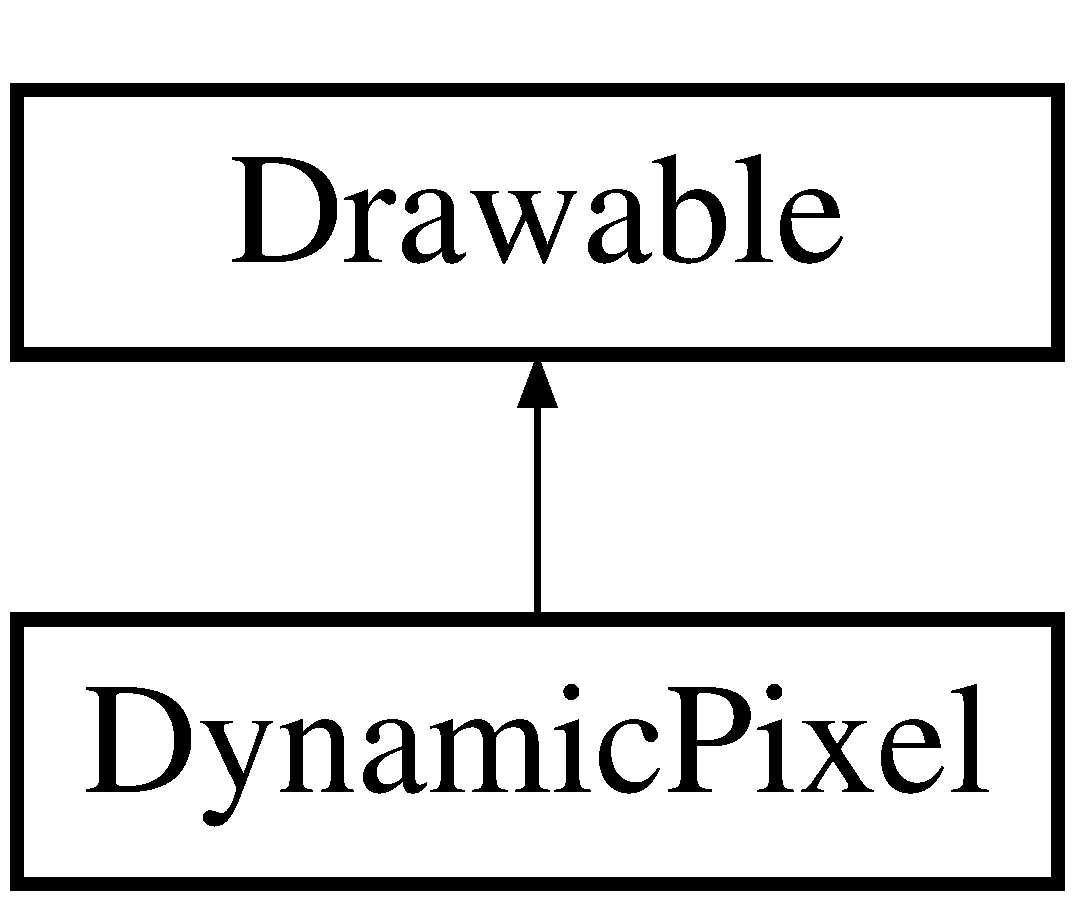
\includegraphics[height=2.000000cm]{class_dynamic_pixel}
\end{center}
\end{figure}
\subsection*{Public Member Functions}
\begin{DoxyCompactItemize}
\item 
\mbox{\Hypertarget{class_dynamic_pixel_a67e9d3edba68ecf4072be4a7e074f15d}\label{class_dynamic_pixel_a67e9d3edba68ecf4072be4a7e074f15d}} 
void {\bfseries draw} (sf\+::\+Render\+Target \&target, sf\+::\+Render\+States states) const
\end{DoxyCompactItemize}
\subsection*{Protected Attributes}
\begin{DoxyCompactItemize}
\item 
\mbox{\Hypertarget{class_dynamic_pixel_aca813100b6b0eb003c28fab84f51a0df}\label{class_dynamic_pixel_aca813100b6b0eb003c28fab84f51a0df}} 
sf\+::\+Vector2f {\bfseries m\+\_\+\+Velocity}
\item 
\mbox{\Hypertarget{class_dynamic_pixel_a428e452a17c872985594b80ecae06d80}\label{class_dynamic_pixel_a428e452a17c872985594b80ecae06d80}} 
float {\bfseries m\+\_\+\+Life\+Time}
\item 
\mbox{\Hypertarget{class_dynamic_pixel_aae21ebb04116b84913e87cf5310c8b23}\label{class_dynamic_pixel_aae21ebb04116b84913e87cf5310c8b23}} 
sf\+::\+Vertex {\bfseries m\+\_\+\+Vertex}
\end{DoxyCompactItemize}


The documentation for this class was generated from the following file\+:\begin{DoxyCompactItemize}
\item 
include/\hyperlink{_dynamic_pixel_8h}{Dynamic\+Pixel.\+h}\end{DoxyCompactItemize}

\hypertarget{class_dynamic_pixel_system}{}\section{Dynamic\+Pixel\+System Class Reference}
\label{class_dynamic_pixel_system}\index{Dynamic\+Pixel\+System@{Dynamic\+Pixel\+System}}
Inheritance diagram for Dynamic\+Pixel\+System\+:\begin{figure}[H]
\begin{center}
\leavevmode
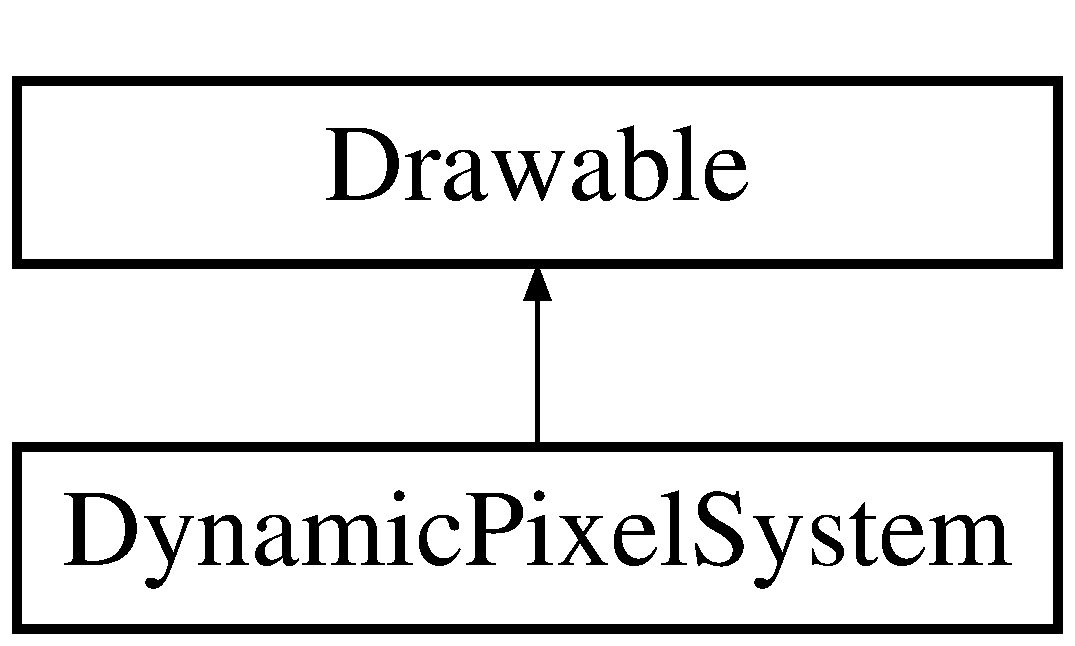
\includegraphics[height=2.000000cm]{class_dynamic_pixel_system}
\end{center}
\end{figure}
\subsection*{Public Member Functions}
\begin{DoxyCompactItemize}
\item 
\mbox{\Hypertarget{class_dynamic_pixel_system_a2797dc7b84f091dc26d8810a85d3c2ed}\label{class_dynamic_pixel_system_a2797dc7b84f091dc26d8810a85d3c2ed}} 
void {\bfseries draw} (sf\+::\+Render\+Target \&target, sf\+::\+Render\+States states) const
\end{DoxyCompactItemize}


The documentation for this class was generated from the following file\+:\begin{DoxyCompactItemize}
\item 
include/\hyperlink{_dynamic_pixel_system_8h}{Dynamic\+Pixel\+System.\+h}\end{DoxyCompactItemize}

\hypertarget{class_game}{}\section{Game Class Reference}
\label{class_game}\index{Game@{Game}}


A game scene that runs the rocket battle game.  




{\ttfamily \#include $<$Game.\+h$>$}



Inheritance diagram for Game\+:\nopagebreak
\begin{figure}[H]
\begin{center}
\leavevmode
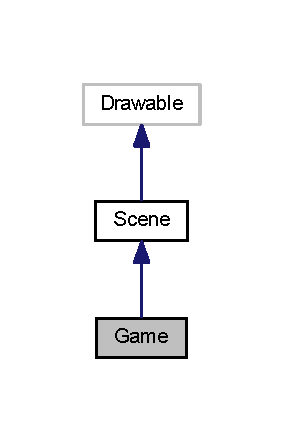
\includegraphics[width=136pt]{class_game__inherit__graph}
\end{center}
\end{figure}


Collaboration diagram for Game\+:\nopagebreak
\begin{figure}[H]
\begin{center}
\leavevmode
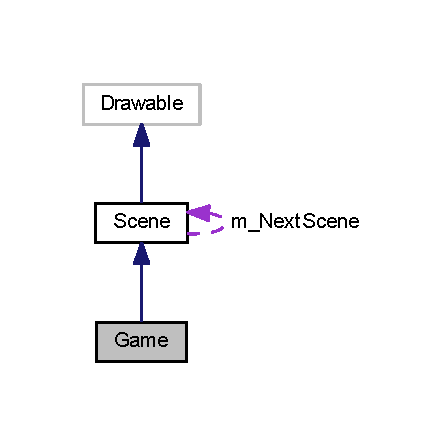
\includegraphics[width=213pt]{class_game__coll__graph}
\end{center}
\end{figure}
\subsection*{Public Member Functions}
\begin{DoxyCompactItemize}
\item 
\hyperlink{class_game_acfaa5dfffe755ef1b09948e9074189b5}{Game} (sf\+::\+Vector2u p\+\_\+\+Window\+Size)
\item 
void \hyperlink{class_game_a6ccc7e91593f06a0e722cc419016a237}{handle\+Keyboard\+Input} (int p\+\_\+\+Key)
\item 
void \hyperlink{class_game_a1c0ddbb7a468997249acbdd6cf2dbe34}{handle\+Mouse\+Input} (sf\+::\+Mouse\+::\+Button p\+\_\+\+Button)
\item 
void \hyperlink{class_game_a3fd12339411955db6a5445ba213ef293}{update} (float p\+\_\+\+Time\+Step)
\item 
void \hyperlink{class_game_a143d1a2f8a527db60f1fe47ab3d854a7}{draw} (sf\+::\+Render\+Target \&target, sf\+::\+Render\+States states) const
\end{DoxyCompactItemize}
\subsection*{Additional Inherited Members}


\subsection{Detailed Description}
A game scene that runs the rocket battle game. 

\subsection{Constructor \& Destructor Documentation}
\mbox{\Hypertarget{class_game_acfaa5dfffe755ef1b09948e9074189b5}\label{class_game_acfaa5dfffe755ef1b09948e9074189b5}} 
\index{Game@{Game}!Game@{Game}}
\index{Game@{Game}!Game@{Game}}
\subsubsection{\texorpdfstring{Game()}{Game()}}
{\footnotesize\ttfamily Game\+::\+Game (\begin{DoxyParamCaption}\item[{sf\+::\+Vector2u}]{p\+\_\+\+Window\+Size }\end{DoxyParamCaption})}

Constructor 
\begin{DoxyParams}[1]{Parameters}
\mbox{\tt in}  & {\em p\+\_\+\+Window\+Size} & Initial window size \\
\hline
\end{DoxyParams}


\subsection{Member Function Documentation}
\mbox{\Hypertarget{class_game_a143d1a2f8a527db60f1fe47ab3d854a7}\label{class_game_a143d1a2f8a527db60f1fe47ab3d854a7}} 
\index{Game@{Game}!draw@{draw}}
\index{draw@{draw}!Game@{Game}}
\subsubsection{\texorpdfstring{draw()}{draw()}}
{\footnotesize\ttfamily void Game\+::draw (\begin{DoxyParamCaption}\item[{sf\+::\+Render\+Target \&}]{target,  }\item[{sf\+::\+Render\+States}]{states }\end{DoxyParamCaption}) const\hspace{0.3cm}{\ttfamily [virtual]}}

Draw 
\begin{DoxyParams}[1]{Parameters}
\mbox{\tt in,out}  & {\em target} & Render target to draw to \\
\hline
\mbox{\tt in}  & {\em states} & Render state \\
\hline
\end{DoxyParams}


Implements \hyperlink{class_scene_ac3fd1d41fa7b7516eeff009de7550552}{Scene}.

\mbox{\Hypertarget{class_game_a6ccc7e91593f06a0e722cc419016a237}\label{class_game_a6ccc7e91593f06a0e722cc419016a237}} 
\index{Game@{Game}!handle\+Keyboard\+Input@{handle\+Keyboard\+Input}}
\index{handle\+Keyboard\+Input@{handle\+Keyboard\+Input}!Game@{Game}}
\subsubsection{\texorpdfstring{handle\+Keyboard\+Input()}{handleKeyboardInput()}}
{\footnotesize\ttfamily void Game\+::handle\+Keyboard\+Input (\begin{DoxyParamCaption}\item[{int}]{p\+\_\+\+Key }\end{DoxyParamCaption})\hspace{0.3cm}{\ttfamily [virtual]}}

handle keyboard events 
\begin{DoxyParams}[1]{Parameters}
\mbox{\tt in}  & {\em p\+\_\+\+Key} & the key that was pressed \\
\hline
\end{DoxyParams}


Implements \hyperlink{class_scene_a182f90e2638c0da6a8ba2eab7cdc73ae}{Scene}.

\mbox{\Hypertarget{class_game_a1c0ddbb7a468997249acbdd6cf2dbe34}\label{class_game_a1c0ddbb7a468997249acbdd6cf2dbe34}} 
\index{Game@{Game}!handle\+Mouse\+Input@{handle\+Mouse\+Input}}
\index{handle\+Mouse\+Input@{handle\+Mouse\+Input}!Game@{Game}}
\subsubsection{\texorpdfstring{handle\+Mouse\+Input()}{handleMouseInput()}}
{\footnotesize\ttfamily void Game\+::handle\+Mouse\+Input (\begin{DoxyParamCaption}\item[{sf\+::\+Mouse\+::\+Button}]{p\+\_\+\+Button }\end{DoxyParamCaption})\hspace{0.3cm}{\ttfamily [virtual]}}

handle mouse button events 
\begin{DoxyParams}[1]{Parameters}
\mbox{\tt in}  & {\em p\+\_\+\+Button} & the button that was pressed \\
\hline
\end{DoxyParams}


Implements \hyperlink{class_scene_ad9240c92a58c4dba4c2409ec8bcff686}{Scene}.

\mbox{\Hypertarget{class_game_a3fd12339411955db6a5445ba213ef293}\label{class_game_a3fd12339411955db6a5445ba213ef293}} 
\index{Game@{Game}!update@{update}}
\index{update@{update}!Game@{Game}}
\subsubsection{\texorpdfstring{update()}{update()}}
{\footnotesize\ttfamily void Game\+::update (\begin{DoxyParamCaption}\item[{float}]{p\+\_\+\+Time\+Step }\end{DoxyParamCaption})\hspace{0.3cm}{\ttfamily [virtual]}}

update the menu 
\begin{DoxyParams}[1]{Parameters}
\mbox{\tt in}  & {\em p\+\_\+\+Time\+Step} & time elapsed since last frame \\
\hline
\end{DoxyParams}


Implements \hyperlink{class_scene_a461d21cd952c7dd0556850a3fc95a760}{Scene}.



The documentation for this class was generated from the following file\+:\begin{DoxyCompactItemize}
\item 
include/\hyperlink{_game_8h}{Game.\+h}\end{DoxyCompactItemize}

\hypertarget{class_terrain}{}\section{Terrain Class Reference}
\label{class_terrain}\index{Terrain@{Terrain}}
Inheritance diagram for Terrain\+:\begin{figure}[H]
\begin{center}
\leavevmode
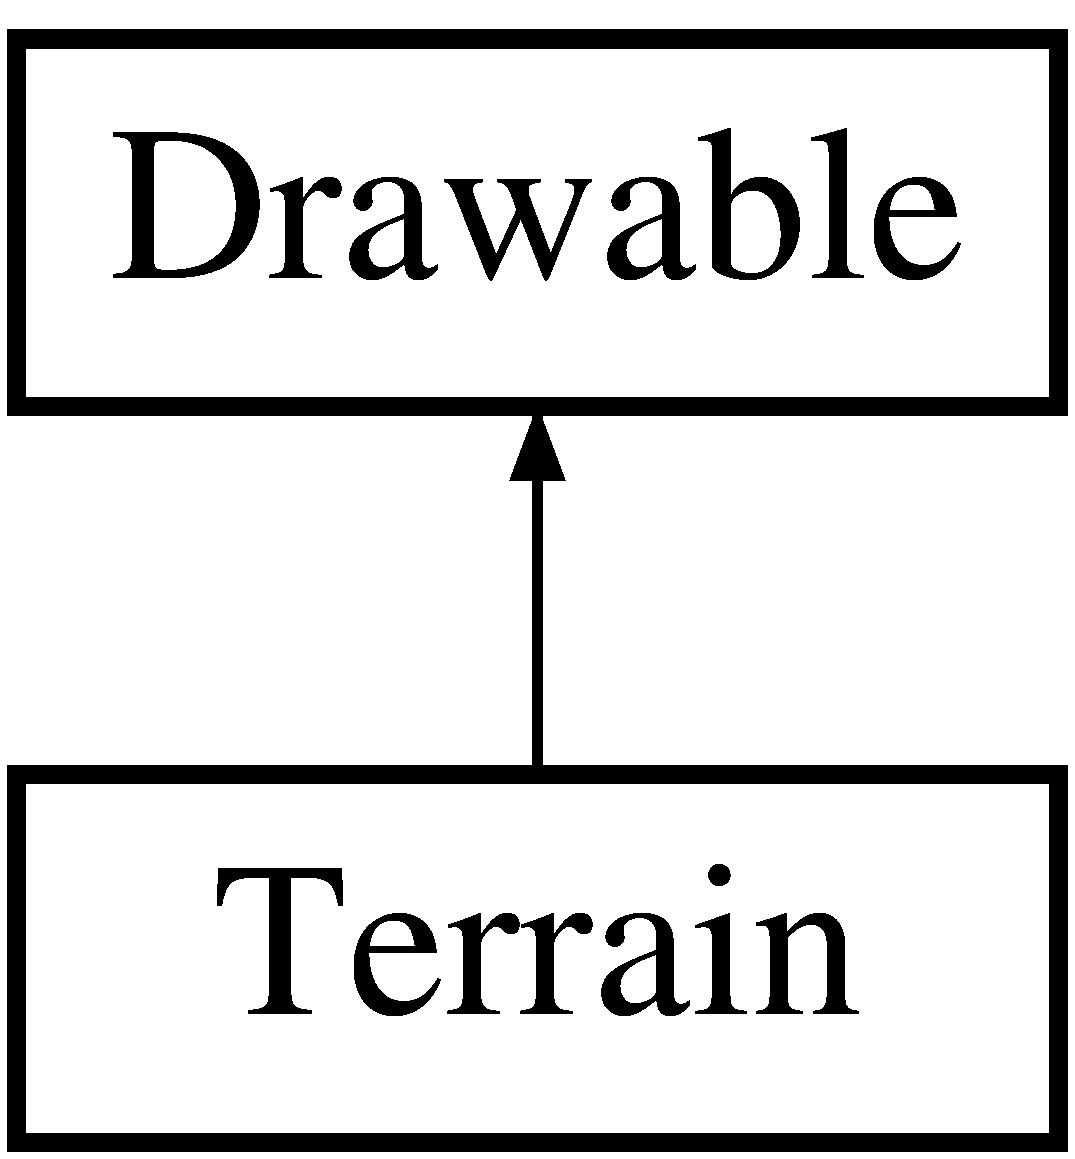
\includegraphics[height=2.000000cm]{class_terrain}
\end{center}
\end{figure}
\subsection*{Public Member Functions}
\begin{DoxyCompactItemize}
\item 
\mbox{\Hypertarget{class_terrain_ab42c4af61b057ccc1af4f2ebbfefa550}\label{class_terrain_ab42c4af61b057ccc1af4f2ebbfefa550}} 
void {\bfseries Load\+Terrain} (sf\+::\+Texture $\ast$p\+\_\+\+Texture)
\item 
\mbox{\Hypertarget{class_terrain_a728b4b72b41aaf1ed463652737b81b37}\label{class_terrain_a728b4b72b41aaf1ed463652737b81b37}} 
sf\+::\+Vector2f {\bfseries Get\+Normal} (unsigned int p\+\_\+X, unsigned int p\+\_\+Y, int p\+\_\+\+Radius)
\item 
\mbox{\Hypertarget{class_terrain_a1929db8af46f2b4a1a053ac33b495bb1}\label{class_terrain_a1929db8af46f2b4a1a053ac33b495bb1}} 
void {\bfseries Subtract\+Shape} (sf\+::\+Shape $\ast$p\+\_\+\+Shape)
\item 
\mbox{\Hypertarget{class_terrain_a46d26ac3525b10ca6bbf065b2627c2b6}\label{class_terrain_a46d26ac3525b10ca6bbf065b2627c2b6}} 
void {\bfseries draw} (sf\+::\+Render\+Target \&target, sf\+::\+Render\+States states) const
\end{DoxyCompactItemize}


The documentation for this class was generated from the following file\+:\begin{DoxyCompactItemize}
\item 
include/\hyperlink{_terrain_8h}{Terrain.\+h}\end{DoxyCompactItemize}

\hypertarget{class_texture_loader}{}\section{Texture\+Loader Class Reference}
\label{class_texture_loader}\index{Texture\+Loader@{Texture\+Loader}}


A singleton loader class that prevents any unnecessary copying of potentially large texture files.  




{\ttfamily \#include $<$Texture\+Loader.\+h$>$}

\subsection*{Public Member Functions}
\begin{DoxyCompactItemize}
\item 
sf\+::\+Texture $\ast$ \hyperlink{class_texture_loader_ad0e763368d9e1ce26b25819113685b28}{get\+Texture} (const std\+::string \&p\+\_\+\+Key)
\item 
void \hyperlink{class_texture_loader_a7e9ef47fb129ac6accf99ec1548c3f6a}{load\+Textures} (const std\+::string \&p\+\_\+\+File\+Path)
\item 
\mbox{\Hypertarget{class_texture_loader_a8e89f35e81bf1cfdd739d91ec0f00831}\label{class_texture_loader_a8e89f35e81bf1cfdd739d91ec0f00831}} 
\hyperlink{class_texture_loader_a8e89f35e81bf1cfdd739d91ec0f00831}{Texture\+Loader} (\hyperlink{class_texture_loader}{Texture\+Loader} const \&)=delete
\begin{DoxyCompactList}\small\item\em prevents the creation of multiple texture loaders \end{DoxyCompactList}\item 
\mbox{\Hypertarget{class_texture_loader_a137de3f6a2f013406d5dcf76d7d4b901}\label{class_texture_loader_a137de3f6a2f013406d5dcf76d7d4b901}} 
\hyperlink{class_texture_loader}{Texture\+Loader} \& \hyperlink{class_texture_loader_a137de3f6a2f013406d5dcf76d7d4b901}{operator=} (\hyperlink{class_texture_loader}{Texture\+Loader} const \&)=delete
\begin{DoxyCompactList}\small\item\em prevents the creation of multiple texture loaders \end{DoxyCompactList}\end{DoxyCompactItemize}
\subsection*{Static Public Member Functions}
\begin{DoxyCompactItemize}
\item 
\mbox{\Hypertarget{class_texture_loader_a530f60fd59904b00f0847f716afe51ab}\label{class_texture_loader_a530f60fd59904b00f0847f716afe51ab}} 
static \hyperlink{class_texture_loader}{Texture\+Loader} $\ast$ \hyperlink{class_texture_loader_a530f60fd59904b00f0847f716afe51ab}{instance} ()
\begin{DoxyCompactList}\small\item\em Returns a pointer to the static texture loader. \end{DoxyCompactList}\end{DoxyCompactItemize}


\subsection{Detailed Description}
A singleton loader class that prevents any unnecessary copying of potentially large texture files. 

\subsection{Member Function Documentation}
\mbox{\Hypertarget{class_texture_loader_ad0e763368d9e1ce26b25819113685b28}\label{class_texture_loader_ad0e763368d9e1ce26b25819113685b28}} 
\index{Texture\+Loader@{Texture\+Loader}!get\+Texture@{get\+Texture}}
\index{get\+Texture@{get\+Texture}!Texture\+Loader@{Texture\+Loader}}
\subsubsection{\texorpdfstring{get\+Texture()}{getTexture()}}
{\footnotesize\ttfamily sf\+::\+Texture$\ast$ Texture\+Loader\+::get\+Texture (\begin{DoxyParamCaption}\item[{const std\+::string \&}]{p\+\_\+\+Key }\end{DoxyParamCaption})}

Returns a texture with the specified key 
\begin{DoxyParams}[1]{Parameters}
\mbox{\tt in}  & {\em p\+\_\+\+Key} & String address to the file \\
\hline
\end{DoxyParams}
\mbox{\Hypertarget{class_texture_loader_a7e9ef47fb129ac6accf99ec1548c3f6a}\label{class_texture_loader_a7e9ef47fb129ac6accf99ec1548c3f6a}} 
\index{Texture\+Loader@{Texture\+Loader}!load\+Textures@{load\+Textures}}
\index{load\+Textures@{load\+Textures}!Texture\+Loader@{Texture\+Loader}}
\subsubsection{\texorpdfstring{load\+Textures()}{loadTextures()}}
{\footnotesize\ttfamily void Texture\+Loader\+::load\+Textures (\begin{DoxyParamCaption}\item[{const std\+::string \&}]{p\+\_\+\+File\+Path }\end{DoxyParamCaption})}

Loads textures from the specified directory 
\begin{DoxyParams}[1]{Parameters}
\mbox{\tt in}  & {\em p\+\_\+\+File\+Path} & Path to a chosen directory \\
\hline
\end{DoxyParams}


The documentation for this class was generated from the following file\+:\begin{DoxyCompactItemize}
\item 
include/\hyperlink{_texture_loader_8h}{Texture\+Loader.\+h}\end{DoxyCompactItemize}

\chapter{File Documentation}
\hypertarget{_dynamic_pixel_8h}{}\section{include/\+Dynamic\+Pixel.h File Reference}
\label{_dynamic_pixel_8h}\index{include/\+Dynamic\+Pixel.\+h@{include/\+Dynamic\+Pixel.\+h}}
{\ttfamily \#include $<$S\+F\+M\+L/\+Graphics.\+hpp$>$}\newline
\subsection*{Classes}
\begin{DoxyCompactItemize}
\item 
class \hyperlink{class_dynamic_pixel}{Dynamic\+Pixel}
\end{DoxyCompactItemize}

\hypertarget{_dynamic_pixel_system_8h}{}\section{include/\+Dynamic\+Pixel\+System.h File Reference}
\label{_dynamic_pixel_system_8h}\index{include/\+Dynamic\+Pixel\+System.\+h@{include/\+Dynamic\+Pixel\+System.\+h}}
{\ttfamily \#include $<$S\+F\+M\+L/\+Graphics.\+hpp$>$}\newline
{\ttfamily \#include \char`\"{}Dynamic\+Pixel.\+h\char`\"{}}\newline
\subsection*{Classes}
\begin{DoxyCompactItemize}
\item 
class \hyperlink{class_dynamic_pixel_system}{Dynamic\+Pixel\+System}
\end{DoxyCompactItemize}

\hypertarget{_game_8h}{}\section{include/\+Game.h File Reference}
\label{_game_8h}\index{include/\+Game.\+h@{include/\+Game.\+h}}
{\ttfamily \#include $<$S\+F\+M\+L\textbackslash{}\+Graphics.\+hpp$>$}\newline
{\ttfamily \#include $<$iostream$>$}\newline
{\ttfamily \#include $<$list$>$}\newline
{\ttfamily \#include \char`\"{}Texture\+Loader.\+h\char`\"{}}\newline
{\ttfamily \#include \char`\"{}Terrain.\+h\char`\"{}}\newline
{\ttfamily \#include \char`\"{}Particle\+System.\+h\char`\"{}}\newline
{\ttfamily \#include \char`\"{}Rocket.\+h\char`\"{}}\newline
{\ttfamily \#include \char`\"{}Aim\+Line.\+h\char`\"{}}\newline
{\ttfamily \#include \char`\"{}Projectile.\+h\char`\"{}}\newline
{\ttfamily \#include \char`\"{}Scene.\+h\char`\"{}}\newline
{\ttfamily \#include \char`\"{}Game\+Over.\+h\char`\"{}}\newline
Include dependency graph for Game.\+h\+:\nopagebreak
\begin{figure}[H]
\begin{center}
\leavevmode
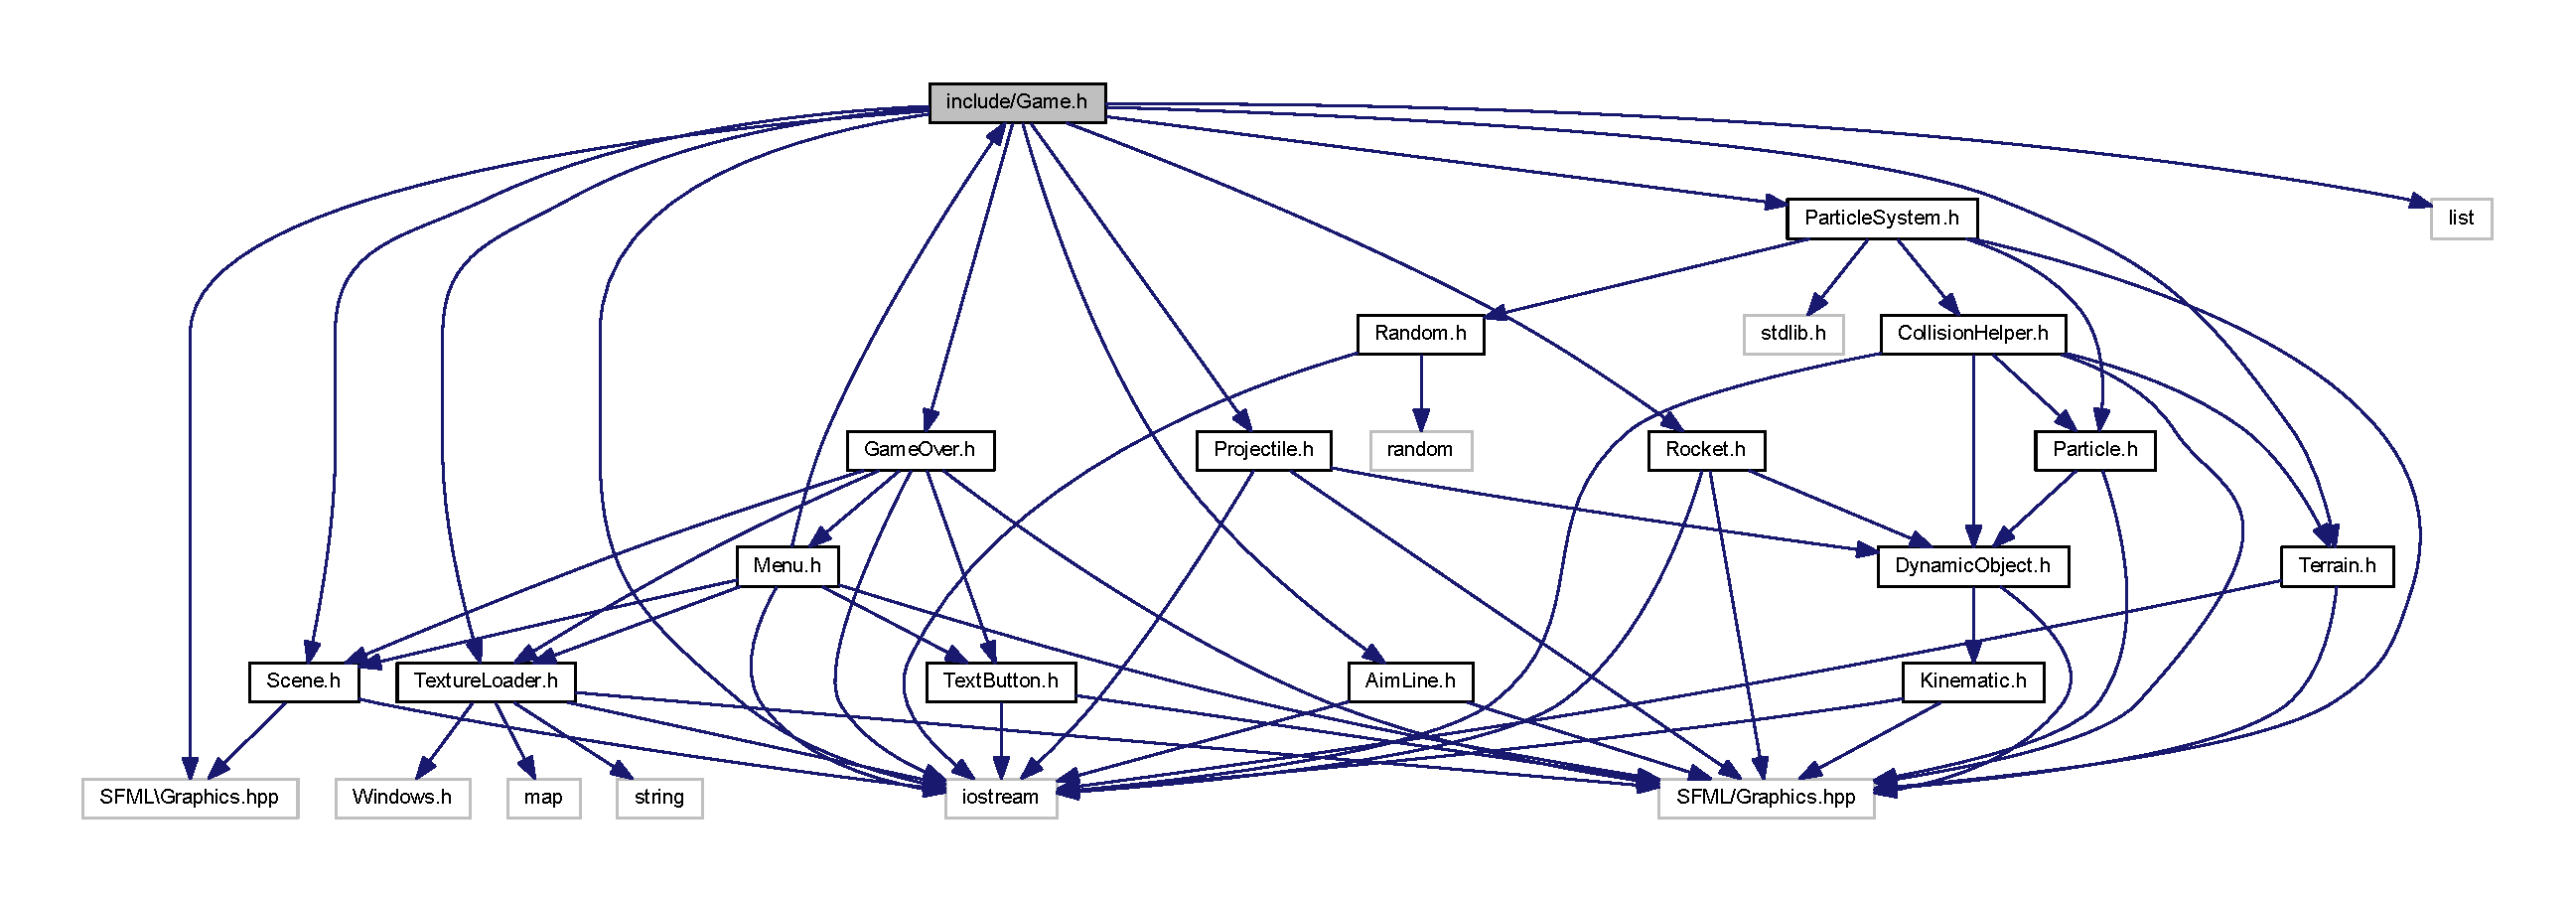
\includegraphics[width=350pt]{_game_8h__incl}
\end{center}
\end{figure}
This graph shows which files directly or indirectly include this file\+:\nopagebreak
\begin{figure}[H]
\begin{center}
\leavevmode
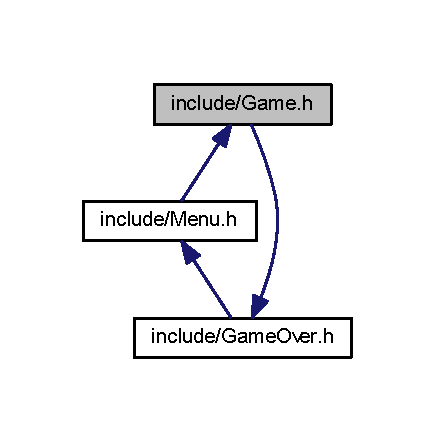
\includegraphics[width=209pt]{_game_8h__dep__incl}
\end{center}
\end{figure}
\subsection*{Classes}
\begin{DoxyCompactItemize}
\item 
class \hyperlink{class_game}{Game}
\begin{DoxyCompactList}\small\item\em A game scene that runs the rocket battle game. \end{DoxyCompactList}\end{DoxyCompactItemize}

\hypertarget{_terrain_8h}{}\section{include/\+Terrain.h File Reference}
\label{_terrain_8h}\index{include/\+Terrain.\+h@{include/\+Terrain.\+h}}
{\ttfamily \#include $<$S\+F\+M\+L/\+Graphics.\+hpp$>$}\newline
\subsection*{Classes}
\begin{DoxyCompactItemize}
\item 
class \hyperlink{class_terrain}{Terrain}
\end{DoxyCompactItemize}

\hypertarget{_texture_loader_8h}{}\section{include/\+Texture\+Loader.h File Reference}
\label{_texture_loader_8h}\index{include/\+Texture\+Loader.\+h@{include/\+Texture\+Loader.\+h}}
{\ttfamily \#include $<$S\+F\+M\+L/\+Graphics.\+hpp$>$}\newline
{\ttfamily \#include $<$map$>$}\newline
{\ttfamily \#include $<$string$>$}\newline
{\ttfamily \#include $<$Windows.\+h$>$}\newline
{\ttfamily \#include $<$iostream$>$}\newline
Include dependency graph for Texture\+Loader.\+h\+:\nopagebreak
\begin{figure}[H]
\begin{center}
\leavevmode
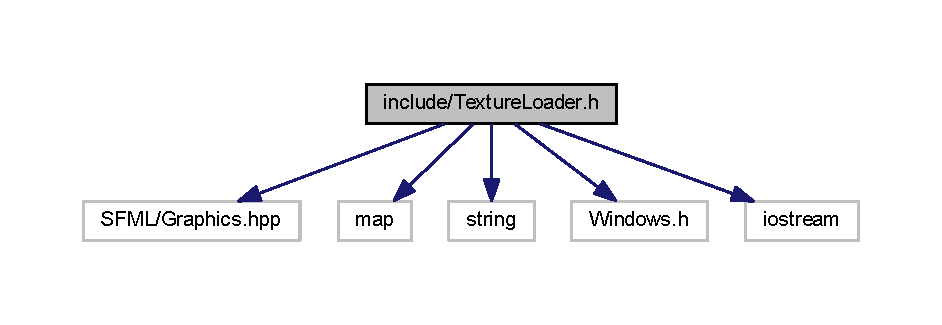
\includegraphics[width=350pt]{_texture_loader_8h__incl}
\end{center}
\end{figure}
This graph shows which files directly or indirectly include this file\+:\nopagebreak
\begin{figure}[H]
\begin{center}
\leavevmode
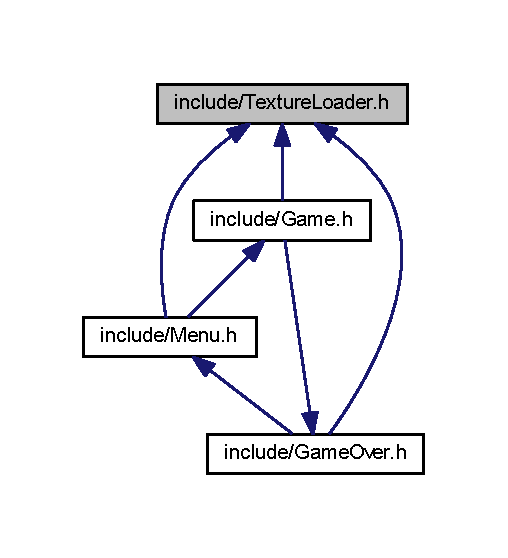
\includegraphics[width=244pt]{_texture_loader_8h__dep__incl}
\end{center}
\end{figure}
\subsection*{Classes}
\begin{DoxyCompactItemize}
\item 
class \hyperlink{class_texture_loader}{Texture\+Loader}
\begin{DoxyCompactList}\small\item\em A singleton loader class that prevents any unnecessary copying of potentially large texture files. \end{DoxyCompactList}\end{DoxyCompactItemize}

%--- End generated contents ---

% Index
\backmatter
\newpage
\phantomsection
\clearemptydoublepage
\addcontentsline{toc}{chapter}{Index}
\printindex

\end{document}
